\documentclass{beamer}

%\usepackage[table]{xcolor}
\mode<presentation> {
  \usetheme{Boadilla}
%  \usetheme{Pittsburgh}
%\usefonttheme[2]{sans}
\renewcommand{\familydefault}{cmss}
%\usepackage{lmodern}
%\usepackage[T1]{fontenc}
%\usepackage{palatino}
%\usepackage{cmbright}
  \setbeamercovered{transparent}
\useinnertheme{rectangles}
}
%\usepackage{normalem}{ulem}
%\usepackage{colortbl, textcomp}
\setbeamercolor{normal text}{fg = black}
\setbeamercolor{structure}{fg = blue}
\definecolor{trial}{cmyk}{1,0,0, 0}
\definecolor{trial2}{cmyk}{0.00,0,1, 0}
\definecolor{darkgreen}{rgb}{0,.4, 0.1}
\definecolor{mygray}{gray}{0.8}
\definecolor{myblack}{rgb}{0, 0, 0}
\usepackage{array}
\beamertemplatesolidbackgroundcolor{white}  \setbeamercolor{alerted
text}{fg=red}

\setbeamertemplate{caption}[numbered]\newcounter{mylastframe}

\usepackage{color}
\usepackage{tikz}
\usetikzlibrary{arrows}
\usepackage{colortbl}
\usepackage{graphicx}
\usepackage{epsfig}

%\usepackage[usenames, dvipsnames]{color}
%\setbeamertemplate{caption}[numbered]\newcounter{mylastframe}c
%\newcolumntype{Y}{\columncolor[cmyk]{0, 0, 1, 0}\raggedright}
%\newcolumntype{C}{\columncolor[cmyk]{1, 0, 0, 0}\raggedright}
%\newcolumntype{G}{\columncolor[rgb]{0, 1, 0}\raggedright}
%\newcolumntype{R}{\columncolor[rgb]{1, 0, 0}\raggedright}

%\begin{beamerboxesrounded}[upper=uppercol,lower=lowercol,shadow=true]{Block}
%$A = B$.
%\end{beamerboxesrounded}}
\renewcommand{\familydefault}{cmss}
%\usepackage[all]{xy}

\usepackage{tikz}
\usepackage{lipsum}

 \newenvironment{changemargin}[3]{%
 \begin{list}{}{%
 \setlength{\topsep}{0pt}%
 \setlength{\leftmargin}{#1}%
 \setlength{\rightmargin}{#2}%
 \setlength{\topmargin}{#3}%
 \setlength{\listparindent}{\parindent}%
 \setlength{\itemindent}{\parindent}%
 \setlength{\parsep}{\parskip}%
 }%
\item[]}{\end{list}}
\usetikzlibrary{arrows}
%\usepackage{palatino}
%\usepackage{eulervm}
\usecolortheme{lily}

\newtheorem{com}{Comment}
\newtheorem{lem} {Lemma}
\newtheorem{prop}{Proposition}
\newtheorem{thm}{Theorem}
\newtheorem{defn}{Definition}
\newtheorem{cor}{Corollary}
\newtheorem{obs}{Observation}
 \numberwithin{equation}{section}


\title[PLSC 43401] % (optional, nur bei langen Titeln nötig)
{Mathematical Foundations of Political Methodology}

\author{Robert Gulotty}
\institute[University of Chicago]{Associate Professor\\Department of Political Science \\  University of Chicago}
\vspace{0.3in}
\date{August 28th, 2017}

\setbeamertemplate{navigation symbols}{}

\begin{document}



\begin{frame}
\titlepage
\end{frame}



\begin{frame}

\begin{itemize}
\item \textcolor{myblack}{Monotone and Inverse Functions}
\item \textcolor{myblack}{Critical Points}
\item \textcolor{myblack}{Second Derivative Test}
\item \textcolor{myblack}{Global Maxima}
\item \textcolor{myblack}{Convex and Concave Functions}
\end{itemize}

\end{frame}



\begin{frame}

\begin{itemize}
\item \textcolor{myblack}{Monotone and Inverse Functions}
\item \textcolor{mygray}{Critical Points}
\item \textcolor{mygray}{Second Derivative Test}
\item \textcolor{mygray}{Global Maxima}
\item \textcolor{mygray}{Convex and Concave Functions}
\end{itemize}

\end{frame}



\begin{frame}
\frametitle{Monotone Functions}

\begin{defn}
Monotonic functions: functions that are either \textit{strictly increasing} or \textit{strictly decreasing}
\end{defn} \pause

\begin{itemize}
\item Strictly increasing: If $x_2>x_1$ then $f(x_2)>f(x_1)$
\item Strictly decreasing: If $x_2>x_1$ then $f(x_2)<f(x_1)$ \pause
\item If $f^\prime(x)>0$ for all $x$, then $f$ is strictly increasing; \\however this is stronger than we need for a function to be strictly increasing (e.g. $f(x)=x^3$)
\item If $f^\prime(x)\geq 0$ for all $x$ and $f^\prime(x)=0$ for only a finite number of $x$, then $f$ is strictly increasing (with strictly decreasing proved similarly)
\end{itemize}

\end{frame}



\begin{frame}
\frametitle{Inverse Functions}

\begin{defn}
Let $f(x)$ be monotonic.  Then for any $y$, $f(x)=y$ has at most one solution. If the solution is written $x=g(y)$, then $g$ is the \textit{inverse function} of $f$, or $$f(g(y))=y \hbox{ and }g(f(x))=x$$
\end{defn} \pause

\ \\Example 1:  Let $f(x)=x^3$; what is the inverse function of $f$? \pause

\ \\Example 2: Let $f(x)=x^{-1}+5$; what is the inverse function of $f$? \pause

\ \\The inverse function is a reflection of the function about the $45^\circ$ line; what's the inverse of the function $\{(1, 2),(2, 3), (3, 4)\}$?

\end{frame}



\begin{frame}
\frametitle{The inverse function rule}

\ \\If $f$ is monotonic with inverse function $g$, and for a given $x$, $f$ is differentiable and $f^\prime(x)\not=0$, then $$f^\prime(y) = \frac{1}{f^\prime(x)}$$ \pause


\ \\This gives us another technique for differentiating things; we could calculate $f^\prime$ directly, or we could calculate $\frac{1}{g^\prime}$

\end{frame}



\begin{frame}

\begin{itemize}
\item \textcolor{mygray}{Monotone and Inverse Functions}
\item \textcolor{myblack}{Critical Points}
\item \textcolor{mygray}{Second Derivative Test}
\item \textcolor{mygray}{Global Maxima}
\item \textcolor{mygray}{Convex and Concave Functions}
\end{itemize}

\end{frame}



\begin{frame}
\frametitle{Critical Points}

\ \\If $f^\prime(x)=0$ then $x$ is called a \textit{critical point}

\begin{itemize}
\item Maximum
\item Minimum
\item Inflection point
\end{itemize}

\begin{center}
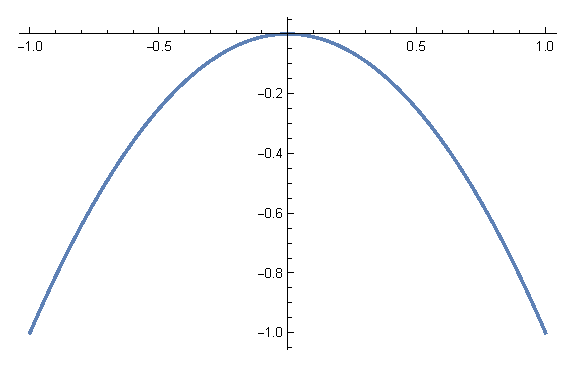
\epsfig{file=max.eps, scale=.32} 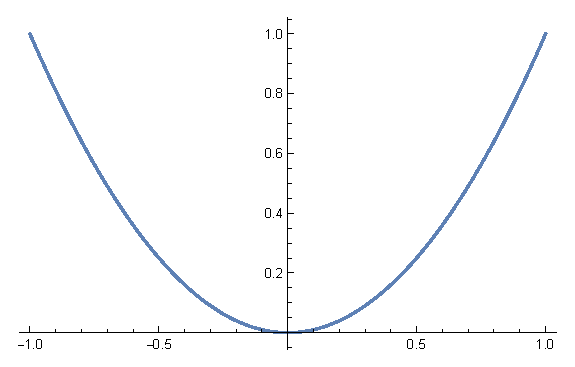
\epsfig{file=min.eps, scale=.32} 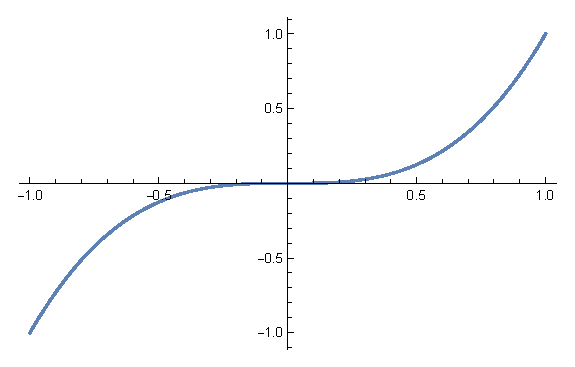
\epsfig{file=inflect.eps, scale=.32}
\end{center}

\end{frame}



\begin{frame}
\frametitle{Critical Points}

One of the main things we use calculus for is to identify and classify critical points \pause

\begin{enumerate}
\item Find $f^\prime(x)$ \pause
\item Find the set of $x$ such that $f^\prime(x)=0$ \pause
\item Intuitively, if $f^\prime(x)$ changes from negative to positive around $x$, then $x$ is a minimum; if it changes from positive to negative then $x$ is a maximum; if it does neither then it's a point of inflection \pause
\item Always remember that without more knowledge of $f$, all we know is that $x$ is a \textit{local} maximum or minimum (or an inflection point); we can't assume that it maximizes or minimizes our function globally
\end{enumerate}

\end{frame}



\begin{frame}

\begin{itemize}
\item \textcolor{mygray}{Monotone and Inverse Functions}
\item \textcolor{mygray}{Critical Points}
\item \textcolor{myblack}{Second Derivative Test}
\item \textcolor{mygray}{Global Maxima}
\item \textcolor{mygray}{Convex and Concave Functions}
\end{itemize}

\end{frame}



\begin{frame}
\frametitle{Second Derivative Test}

Recall that if $f^\prime$ is itself differentiable, then $f$ is \textit{twice differentiable}, and $f^{\prime\prime} = \frac{d^2y}{dx^2}$ is the \textit{second derivative} \pause

\begin{itemize}
\item Suppose that $f^{\prime\prime}(x)$ is positive at some point $x$ \pause
\item This means that the \textit{slope of the slope} of $f$ is increasing at $x$ \pause
\item This means that either:

\begin{itemize}

\item If $f$ is increasing then it's increasing at an increasingly faster rate at $x$ \pause
\item If $f$ is decreasing then it's decreasing at an increasingly slower rate at $x$ \pause
\item If $f$ is flat then it's increasing as $x$ increases \pause

\end{itemize}
\item In all of these cases, $f$ lies above its tangent
\end{itemize}

\end{frame}



\begin{frame}
\frametitle{Second Derivative Test}

\begin{itemize}

\item[A] If $f$ is increasing then it's increasing at an increasingly faster rate at $x$ \pause
\item[B] If $f$ is decreasing then it's decreasing at an increasingly slower rate at $x$ \pause
\item[C] If $f$ is flat then it's increasing as $x$ increases

\end{itemize}

\vspace{.2in}
\begin{center}
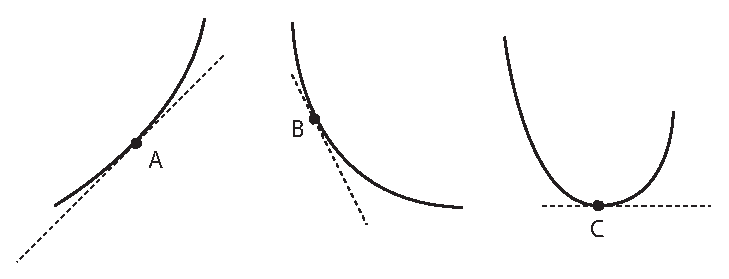
\epsfig{file=convex.eps, scale=.75}
\end{center}

\end{frame}



\begin{frame}
\frametitle{Second Derivative Test}

\begin{itemize}
\item For any critical point, $x^*$, calculate $f^{\prime\prime}(x^*)$ \pause

\begin{itemize}
\item If $f^{\prime\prime}(x^*)>0$ then $x^*$ is a local minimum \pause
\item If $f^{\prime\prime}(x^*)<0$ then $x^*$ is a local maximum \pause

\item If $f^{\prime\prime}(x^*)=0$ then we don't know what $x^*$ is; we have to examine our function around $x^*$ \pause

\end{itemize}

\item $f^\prime(x)=0$ is our first-order condition; conditions on $f^{\prime\prime}$ are our second-order conditions \pause

\end{itemize}

\ \\Find and classify the critical points of $x^3-3x$, and then use this information to plot out the function

\end{frame}



\begin{frame}

\begin{itemize}
\item \textcolor{mygray}{Monotone and Inverse Functions}
\item \textcolor{mygray}{Critical Points}
\item \textcolor{mygray}{Second Derivative Test}
\item \textcolor{myblack}{Global Maxima}
\item \textcolor{mygray}{Convex and Concave Functions}
\end{itemize}

\end{frame}



\begin{frame}
\frametitle{Global Maxima}

\ \\If a local maximum $x^*$ has the additional property that $f(x^*)\geq f(x)$ for all $x\in \mathbb{R}$ then $x^*$ is a global maximum \pause

\ \\Important points about global maxima that we will use shortly \pause

\begin{itemize}
\item Suppose that $g(x)=H(f(x))$ where $H$ is a \textit{strictly increasing function}.  Then if $f$ has a global maximum at $x^*$, $g(x)$ also has a global maximum at $x^*$ \pause
\begin{itemize}
\item If $f(x^*)\geq f(x)$ for all $x$, then $H(f(x^*))\geq H(f(x))$ for all $x$, since $H$ is a strictly increasing function \pause
\item It can be useful to take a log; if $x^*$ globally maximizes log$(f(x))$ then $x^*$ also maximizes $f(x)$ \pause
\end{itemize}

\item If $x^*$ is the global max of $f(x)$ then $x^*$ is the global minimum of $-f(x)$ \pause
\end{itemize}

\end{frame}



\begin{frame}
\frametitle{Boundary Conditions \& Asymptotes}

\ \\ If the domain of a function is bounded, it may be the case that a global maximum is attained at one of the boundaries, even when the first-order condition at that point is not satisfied; use common sense and try to have a sense of what your function looks like -- some problems are best solved without calculus. \pause

\begin{theorem}
The extreme value theorem:  any continuous function on a closed and bounded interval attains a global maximum and minimum
\end{theorem} \pause

\ \\Some functions tend to a straight line for all very large values of $|x|$ and / or  $|y|$; it can be useful to know this \pause

\begin{itemize}
\item $y={\frac{1}{x}}$ ($x>0$) has a $x-$ and $y-$ asymptotes equal to the axes \pause
\item What are the asymptotes for $y=x-{\frac{1}{x}}$ %has asymptotes equal to the y axis and the line y=x
\end{itemize}

\end{frame}



\begin{frame}

\begin{itemize}
\item \textcolor{mygray}{Monotone and Inverse Functions}
\item \textcolor{mygray}{Critical Points}
\item \textcolor{mygray}{Second Derivative Test}
\item \textcolor{mygray}{Global Maxima}
\item \textcolor{myblack}{Convex and Concave Functions}
\end{itemize}

\end{frame}



\begin{frame}
\frametitle{Convexity and Concavity}

Convex and concave functions guarantee that local optima are global optima, and are commonly encountered. \pause
 
\begin{defn}
A set is \textit{convex} if the line segment connecting any two points in the set is entirely contained within the set
\end{defn}

\begin{center}
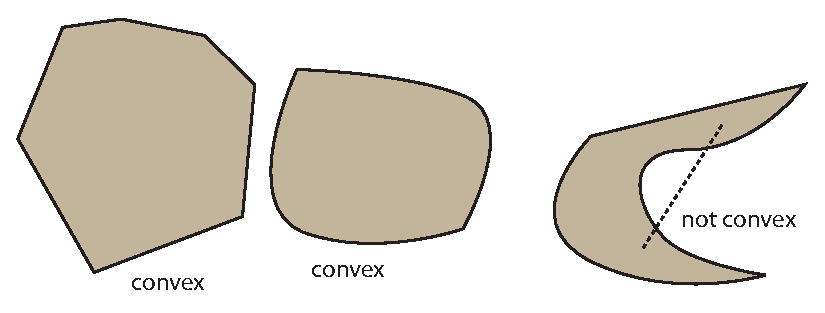
\epsfig{file=convexSet.eps, scale=.65}
\end{center}

\end{frame}



\begin{frame}
\frametitle{Convex Function}

\begin{defn}
$f$ is a convex function if and only if for all real numbers $A, B$ and all $0\leq \alpha \leq 1$, 
$$\alpha f(A)+(1-\alpha)f(B)\geq f(\alpha A+(1-\alpha)B)$$
\end{defn}

\begin{center}
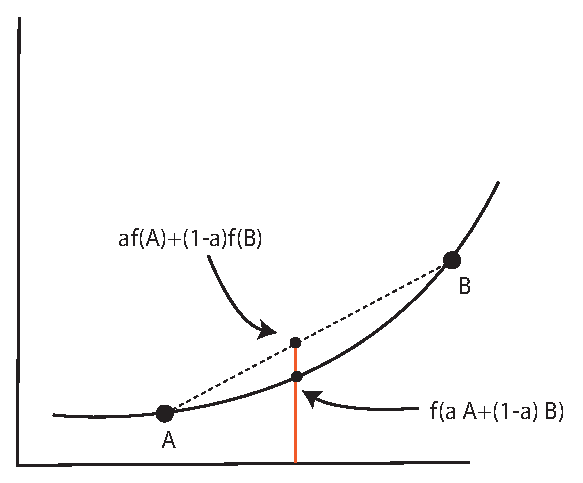
\epsfig{file=convexFunction.eps, scale=.65}
\end{center}

\end{frame}



\begin{frame}
\frametitle{Convex Function}

Convex functions need not be differentiable (e.g. $y=|x|$); the ones we generally encounter are \pause

\begin{itemize}
\item If $f$ is twice differentiable, then $f$ is convex if and only if $f^{\prime\prime}\geq 0$ for all $x$ \pause

\item If $f$ is differentiable then
\begin{itemize}
\item There is either no global minimum, one global minimum, or an interval of global minima \pause
\item There are no local minima that are not global minima \pause
\item Important: if $f^\prime(x^*)=0$ then $x^*$ is a global minimum \pause
\end{itemize}
\item $f$ is \textit{strictly convex} if $\alpha f(A)+(1-\alpha)f(B)> f(\alpha A+(1-\alpha)B)$ when $\alpha\in(0, 1)$
\end{itemize}

\end{frame}



\begin{frame}
\frametitle{Concave Function}

\begin{defn}
$f$ is \textit{concave} if and only if $-f$ is convex: the set of all points on or below $f$ is convex
\end{defn} \pause

\begin{itemize}
\item If $f$ is twice differentiable then $f$ is concave if and only if $f^{\prime\prime}\leq 0$ for all $x$ \pause

\item Important: if $f$ is concave and $f^\prime(x^*)=0$ then $x^*$ is a global maximum

\end{itemize}

\end{frame}



\begin{frame}
\frametitle{Find Maxima/Minima: A Summary}

\begin{itemize}

\item Compute $f^{'}(x)$ and find all $x$ such that $f^{'}(x) = 0$; \pause

\item Conduct second derivative test, compute $f^{''}(x)$ for all $x$ such that $f^{'}(x) = 0$; \pause

\begin{itemize}
\item $f^{''}(x) > 0$, then, it's a local minimum; \pause
\item $f^{''}(x) < 0$, then, it's a local maximum; \pause
\item $f^{''}(x) = 0$, then, undecided. \pause
\end{itemize}

\item Finally, check boundary points, and determine global maxima or minima.

\end{itemize}

\end{frame}



\begin{frame}
\frametitle{Example 1: $f(x) = -x^2$,  $x \in [-3, 3] $}

	1) Critical Value:

	\begin{eqnarray}
	f^{'}(x) & = & - 2 x \nonumber \\
	0 & = & - 2 x^{*} \nonumber \\
	x^{*} & = & 0 \nonumber 
	\end{eqnarray} \pause

	2) Second Derivative: 

	\begin{eqnarray}
	f^{'}(x) & = & - 2x \nonumber \\
	f^{''}(x)  & = & - 2 \nonumber 
	\end{eqnarray}
	$f^{''}(x)< 0$, local maximum


\end{frame}

\begin{frame}
\frametitle{Example 1: $f(x) = -x^2$,  $x \in [-3, 3] $}

	3) Check end points
	\begin{eqnarray}
	f(0) & = & - 0 ^2 = 0 \nonumber \\
	f(-3) & = & - (-3)^2 = -9 \nonumber \\
	f(3) & = & - (3)^2 = -9 \nonumber 
	\end{eqnarray}

\end{frame}


\begin{frame}
\frametitle{Example 2: $f(x) = x^3$, $x \in [-3, 3] $ }

1) Critical Values: 
\begin{eqnarray}
f^{'}(x) & = & 3x^2 \nonumber \\
0 & = & 3 (x^{*})^{2} \nonumber \\
x^{*} & = & 0 \nonumber 
\end{eqnarray} \pause

2) Second Derivative: 

\begin{eqnarray}
f^{''}(x) & = & 6 x \nonumber \\
f^{''}(0) & = &  0 \nonumber 
\end{eqnarray}
\alert{No information}

\end{frame}



\begin{frame}
\frametitle{Example 2: $f(x) = x^3$, $x \in [-3, 3] $}


3) Check End Points: 

\begin{eqnarray}
f(0) & = & 0^3  = 0 \nonumber \\
f(-3) & = & -3^3 = -27 \nonumber \\
f(3) & = & 3^3 = 27 \nonumber 
\end{eqnarray}

Neither maximum nor minimum, \alert{saddle point} 

\end{frame}



\begin{frame}
\frametitle{Example 3: Spatial Model}
A large literature in Congress supposes legislators and policies can be situated in \alert{policy space} \pause \\

Suppose legislator $i$ and policies $x, i \in \Re$. \pause  \\
Define legislator $i$'s utility as, $U:\Re \rightarrow \Re$, \pause 
\begin{eqnarray}
U_{i} (x) & = & - (x - \mu)^{2}  \nonumber \\ \pause 
U_{i}(x) & = & - x^2 +  2 x \mu  - \mu^2 \nonumber \pause 
\end{eqnarray}
What is $i$'s optimal policy over the range $x \in [\mu- 2, \mu + 2]$? \pause 
\begin{eqnarray}
U_{i}^{'} (x) & = & -2 (x - \mu) \nonumber \\ \pause 
0 & = & -2x^{*} + 2 \mu \nonumber \\ \pause 
x^{*} & = & \mu \nonumber \pause 
\end{eqnarray}

\alert{Second Derivative Test} \pause 
\begin{eqnarray}
U^{''}_{i}(x)  & = & -2 <0  \nonumber \pause 
\end{eqnarray}

We call $\alert{\mu}$ legislator $i$'s \alert{ideal point} 

\end{frame} 

\begin{frame}
\frametitle{Example 3: Spatial Model}

\begin{eqnarray}
U_{i}(\mu) & = & - (\mu - \mu)^2 = 0 \nonumber \\
U_{i}(\mu - 2) & = & - (\mu - 2 - \mu)^2 = -4 \nonumber \\
U_{i} (\mu + 2) & = & - (\mu + 2 - \mu)^2 = -4 \nonumber 
\end{eqnarray}

\alert{Maximize utility at $\mu$}

\end{frame}



\end{document}
